To find the optimal algorithm for handwritten digit recognition the K-NN and Decision trees algorithms will be compared.
In this section the algorithms are compared based on training, classification and success rate.

\subsection{Training}
The K-NN algorithm is a direct comparison of the train data and the test data.
Thus it does not need to build a model.
Instead the K-NN algorithm relies on preprocessing the data.
In terms of speed this is faster as the test data will be preprocessed with the same methods as well.

The decision tree algorithm has to build a model of the training data. 
As shown in section \ref{sec:tree} building the decision tree from the training data of 19 people takes 3056.21 seconds.
It can be assumed that the model will only be built once as a setup and thus the impact of building the model should not be a determining factor.

\subsection{Classification Time}
A big difference between K-NN and decision trees are that K-NN is a brute force comparison.
In figure \ref{fig:algo_compare_timing} is the timing of classification compared.
400 digits of each class were classified using 19 peoples data as training.
Here it is clear that K-NN takes more time to classify the digits.
The tree removes half of the potential comparisons with each decision split which makes it scale well on large datasets.

\begin{figure}[H]
\centering
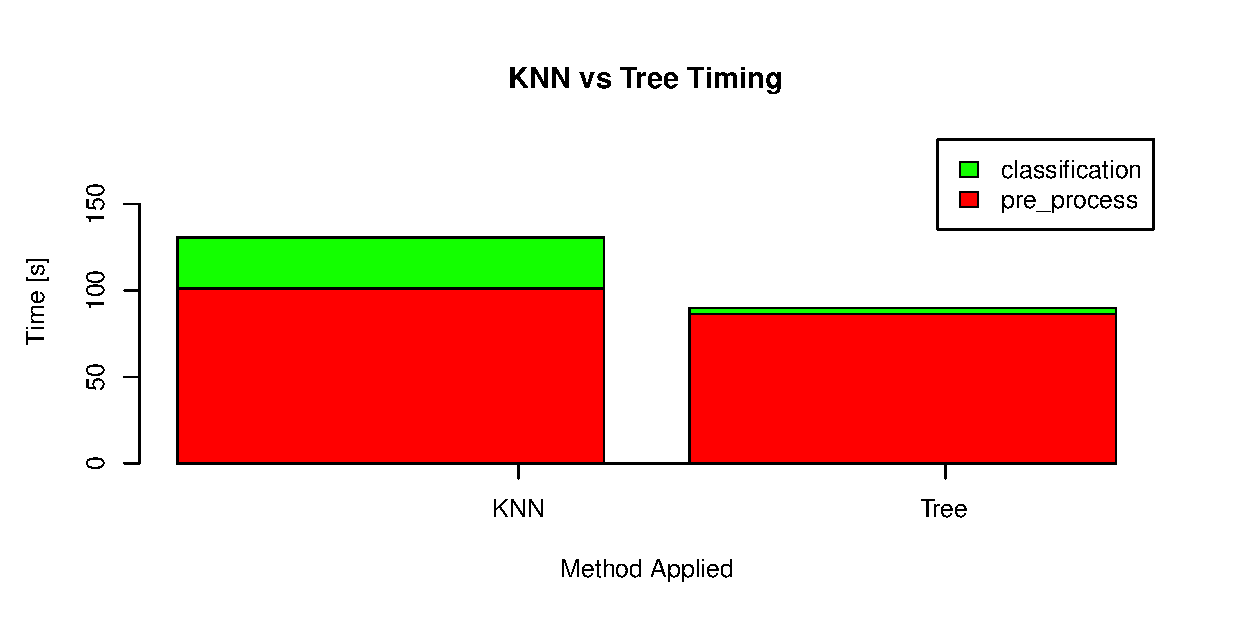
\includegraphics[width=\textwidth]{graphics/algo_compare_timing}
\caption{Classification timing of the two models.}
\label{fig:algo_compare_timing}
\end{figure}
% tree_vs_knn_timing.R

\subsection{Success Rate}
The performance of a classification method is measured in the success rate on the test data.
It can be seen that the decision tree algorithm has a better overall performance.
On the easy problem the K-NN gave a mean success rate of 
85.07\% with a variance of 3.59\(\%^2\)
where the decision tree gave a mean success rate of
86.14\% with a variance of 4.96\(\%^2\). 
In figure \ref{fig:success_comparison_hard} is the algorithms success rate of the hard problem shown.
On the hard problem the K-NN gave a mean success rate of 
70.99\% with a variance of 117.81\(\%^2\)
where the decision tree gave a mean success rate of
72.95\% with a variance of 177.48\(\%^2\), 
making decision trees better at classifications on both problems.
It is noteworthy that in several cases the performance amplify the behaviour from the K-NN test.
Thus cases like G1M1, G2M2 and G7M3, which has a worse than average detection gets worse result than K-NN 
and cases where the performance is better than the average gets a even better detection rate.
This is suspected to be a result of overfitting the model to people with a ``good'' handwriting.
An outlier is G7M1 who has an above average performance in K-NN and gets a much worse performance and G1M3 who gets a better performance.

\begin{figure}[H]
\centering
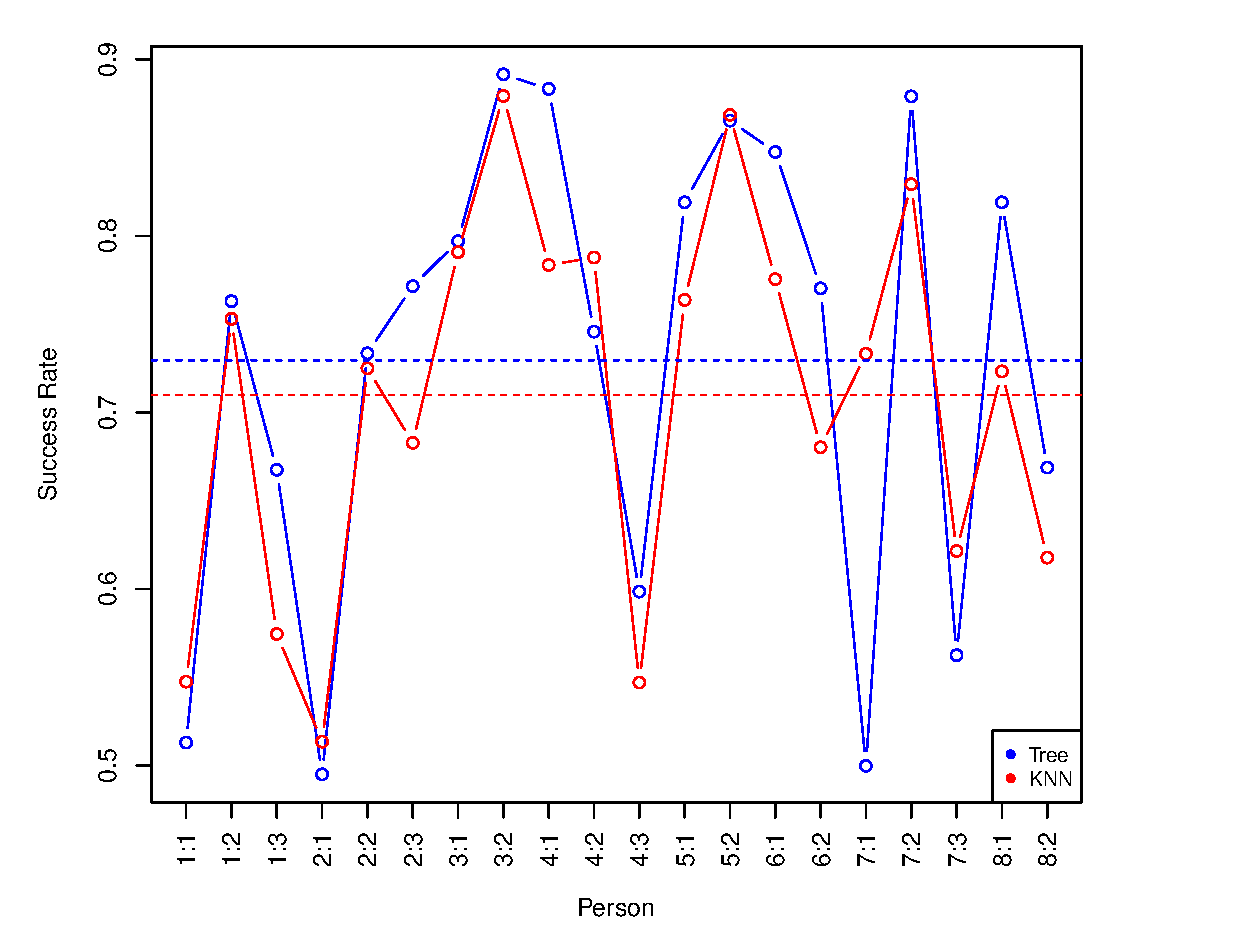
\includegraphics[width=\textwidth]{graphics/success_comp_hard}
\caption{Success for different group members.}
\label{fig:success_comparison_hard}
\end{figure}

